\documentclass{article}

\usepackage{color}
\usepackage{graphicx}
\usepackage{tabularx}


\usepackage{geometry}
 \geometry{
 top=20mm,
 bottom=20mm,
 }


\title{Document de pr\'esentation}
\author{Justal Kevin}
\date{26/09/2015}
\renewcommand{\contentsname}{Table des mati\`eres} 
 
\newcommand\invisiblesection[1]{%
  \refstepcounter{section}%
  \addcontentsline{toc}{section}{\protect\numberline{\thesection}#1}%
  \sectionmark{#1}} 
 
\begin{document}

\begin{center}
\textbf{\Huge{LES ANIMAUX}}
\line(1,0){300}\\
DOSSIER DE CONCEPTION\\
\vspace{3cm}
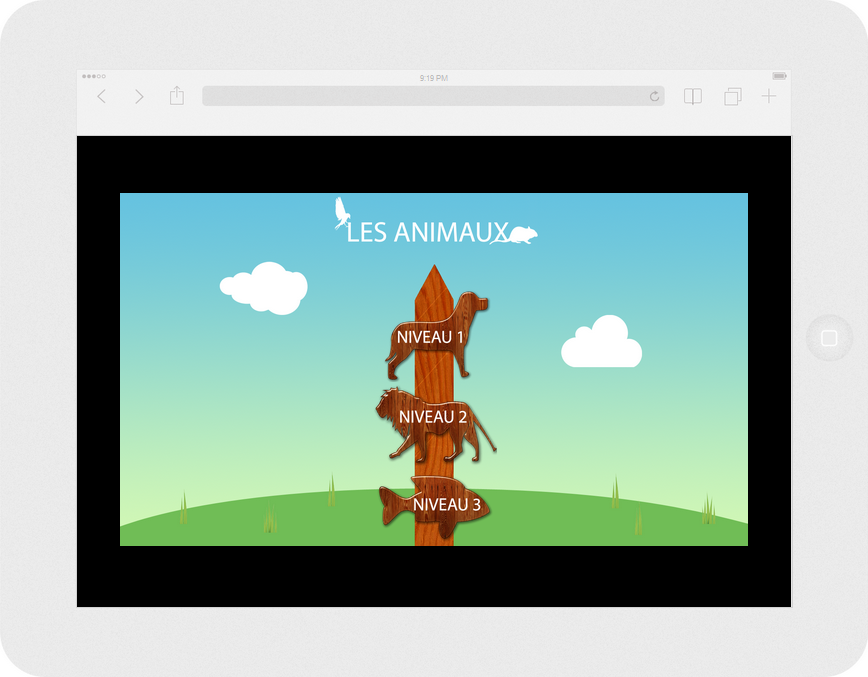
\includegraphics[width=0.8\textwidth]{tablette}\\
\vspace{3cm}
\textbf{Justal Kevin - \color{blue}{\underline{justal@polytech.unice.fr}} \color{black}{- SI5 - IHM}}\\
\textbf{Houda Smach - \color{blue}{\underline{smach.houda@gmail.com}} \color{black}{- SSTIM }}\\
\textbf{Belokogne Ivan - \color{blue}{\underline{bel.ivan@live.com }} \color{black}{- SSTIM }}\\
\vspace{4cm}
\textbf{Encadrant :}\\
\textbf{Jean-Paul Stromboni - \color{blue}{\underline{strombon@polytech.unice.fr}}}
\end{center}

\newpage
\tableofcontents

\newpage

\section{Pr\'esentation de l'application}
\hspace*{0.6cm}Les jeux accessibles sont un bon moyen d'aider le d\'eveloppement intellectuel et psychologique des enfants handicap\'es. C'est pour cela que nous avons d\'ecid\'e de produire un jeu le plus simple possible faisant travailler l'intelligence logico-math\'ematique et corporelle kinesth\'esique des enfants. Le jeu confronte les enfants \`a plusieurs images d'animaux et des cases o\`u chaque animal peut \^etre rang\'e. Les enfants devront donc associer des animaux ayant le m\^eme nombre de pattes, le m\^eme type d'habitation ou encore la m\^eme cat\'egorie (domestique, de la ferme, sauvage).
\section{Structure de l'application}

\subsection{D\'eroulement}

La structure g\'enerale de notre application sera la suivante :
\vspace{0.5cm}\\
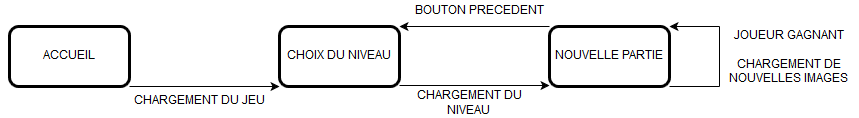
\includegraphics[width=\textwidth]{plan}
\vspace{0.5cm}\\
\hspace*{0.6cm}La structure est volontairement simple afin que toute personne puisse prendre le jeu en main sans aucune indication.\\
Une fois la page d'accueil charg\'ee, le choix des diff\'erents niveaux s'affiche. Lorsque l'utilisateur clique sur l'une des options, le jeu lance le niveau selectionn\'e.\\
Si l'utilisateur d\'ecide d'arr\^eter le jeu ou de changer de niveau, il peut alors revenir au menu du d\'epart en cliquant sur le bouton "retour". 

\subsection{UML}

\begin{center}
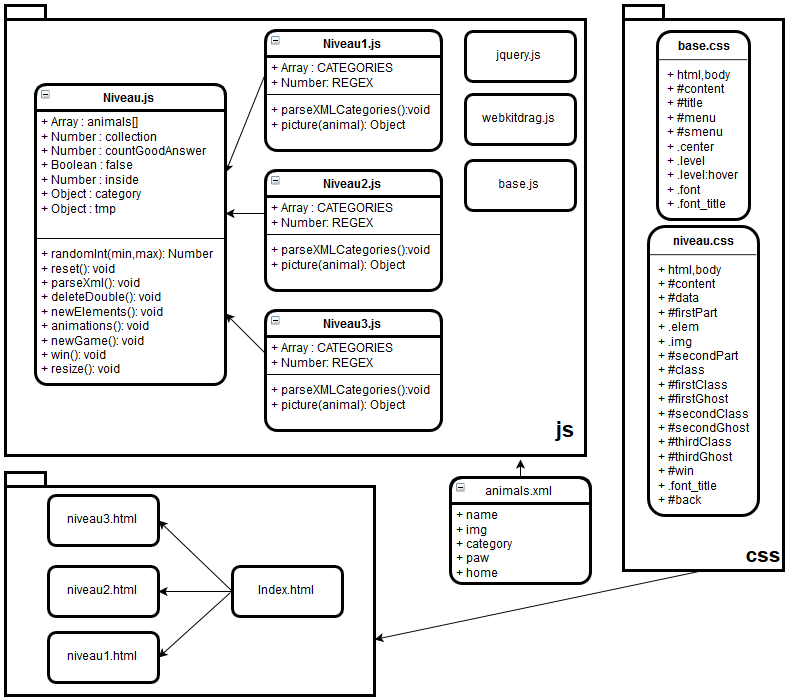
\includegraphics[width=0.8\textwidth]{planUml}\\
\end{center}

\section{Interfaces}
\hspace*{0.6cm}Le jeu dispose de quatre sc\`enes cl\'es qui \`a elles seules suffisent pour d\'ecrire le jeu entier. Dans chaque section du jeu, nous verrons en d\'etail les objectifs et les accomplissements que l'on attend du joueur. 
\subsection{Ecran d'accueil}
\vspace{0.5cm}
\begin{center}
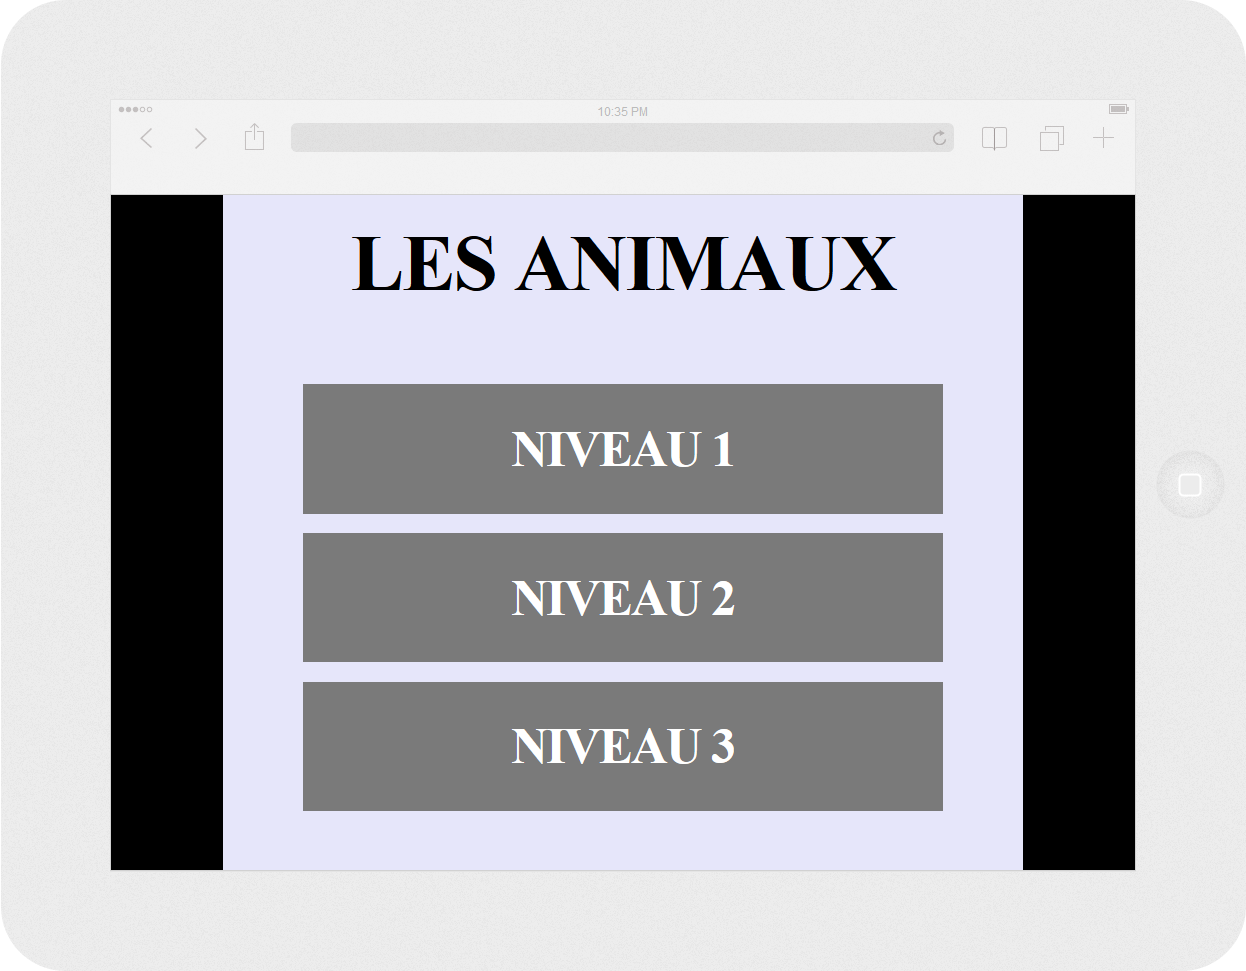
\includegraphics[width=0.6\textwidth]{page1}
\end{center}
\vspace{0.5cm}
\hspace*{0.6cm}Le menu est tr\`es simple, \'epur\'e de tout contenu additionnel inutile. Le texte est \'ecrit tr\`es gros au cas o\`u l'enfant aurait un handicap visuel. De m\^eme pour \'eviter que l'enfant ouvre les options du navigateur au cas o\`u le jeu serait lanc\'e sur un ordinateur, le clic droit a \'et\'e d\'esactiv\'e. Le cursor a aussi \'et\'e modifi\'e, il est beaucoup plus grand que la normal pour l'enfant atteint d'un handicap visuel.
\vspace{0.5cm}\\
\hspace*{0.6cm}Sinon concernant le menu, il y a le minimum d'animation pour que le joueur puisse s'y retrouver. Lorsque le joueur passe la souris sur les diff\'erents niveaux, ces derniers sont surlign\'es et grossis l\'eg\`erement.
\subsection{Niveau 1 - Trier par cat\'egories}
\vspace{0.5cm}
\begin{center}
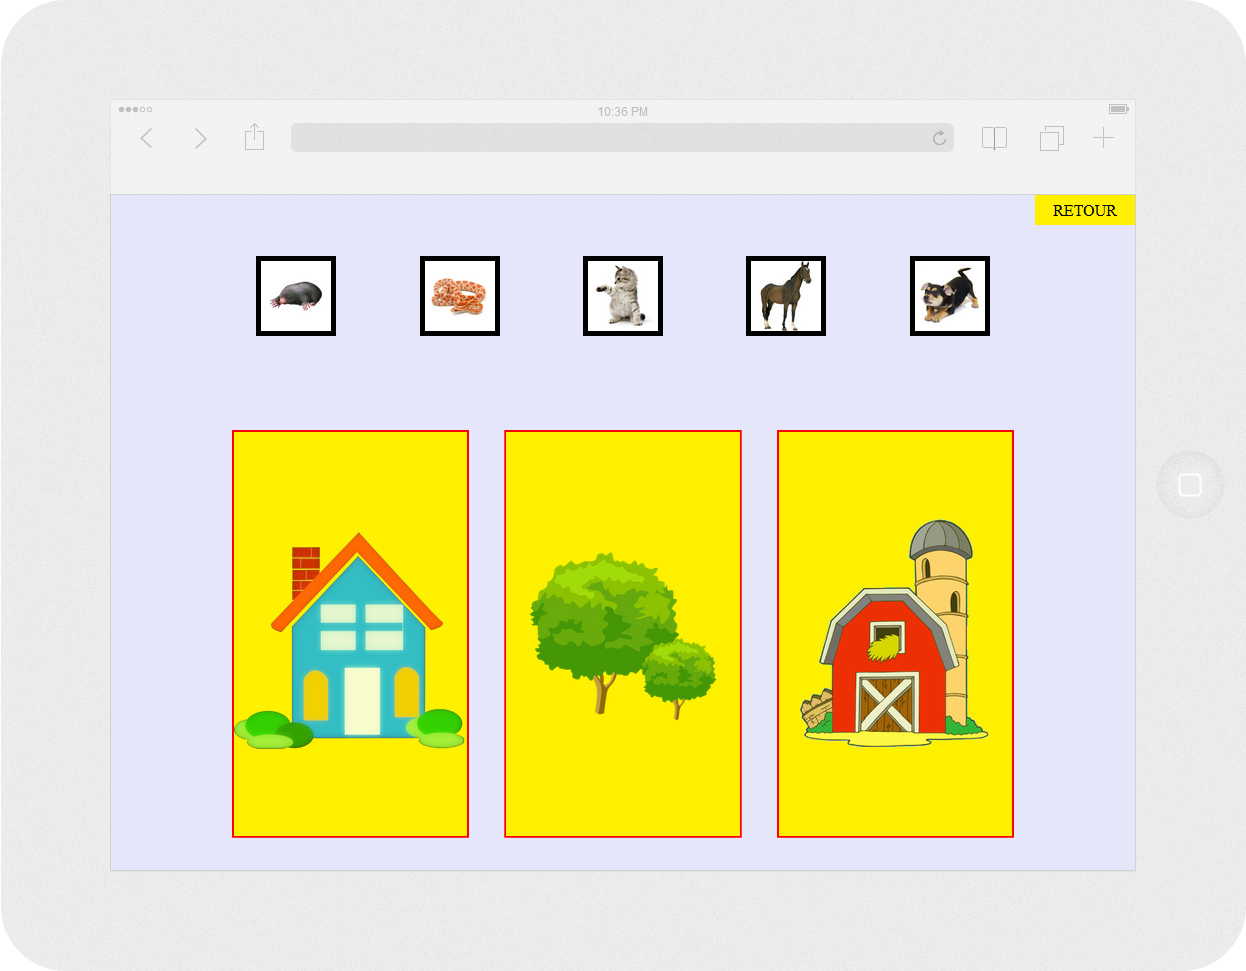
\includegraphics[width=0.6\textwidth]{page2}
\end{center}
\vspace{0.5cm}
\hspace*{0.6cm}Comme l'ensemble du jeu, les niveaux sont eux aussi simplifi\'es au maximum.
Le premier niveau consiste \`a associer les animaux affich\'es \`a leurs cat\'egories respectives. Prenons un exemple, un chat ira dans la cat\'egorie domestique. On glisse alors l'image du chat sur la case jaune qui contient une maison. En cas de bonne r\'eponse, l'image reste dans la case pr\'evue. En cas de mauvaise r\'eponse, l'image retourne \`a son emplacement d'origine.
\subsection{Niveau 2 - Trier par nombre de pattes}
\vspace{0.5cm}
\begin{center}
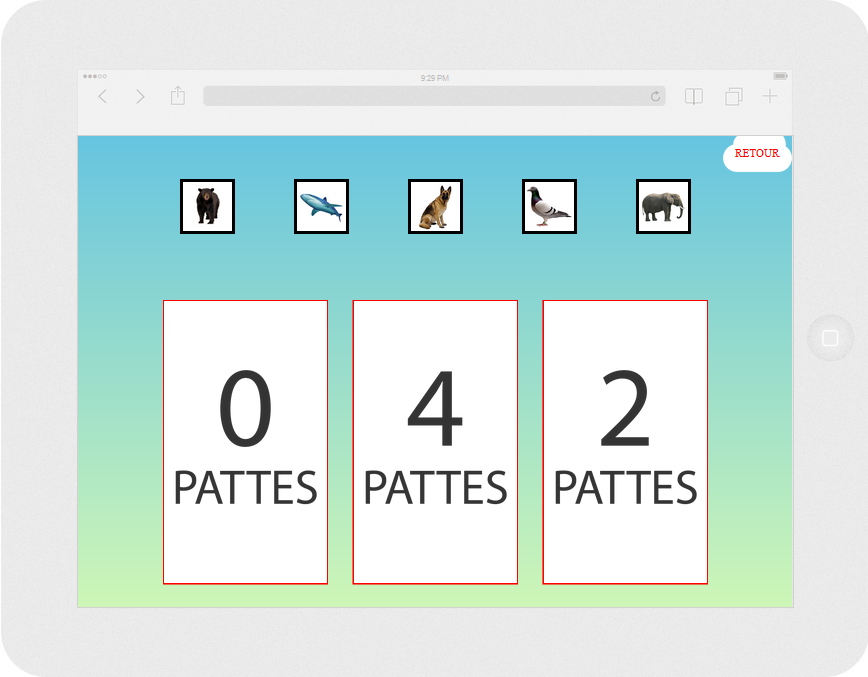
\includegraphics[width=0.6\textwidth]{page3}
\end{center}
\vspace{0.5cm}
\hspace*{0.6cm}Le niveau 2 est semblable au premier dans sa structure mais le jeu est plus difficile que le niveau 1. Dans ce niveau, le joueur doit trier les animaux par nombre de pattes. Par exemple, la case jaune avec le chien est la case qui regroupe les animaux avec 4 pattes comme le chat.
\subsection{Niveau 3 - Trier par habitation}
\vspace{0.5cm}
\begin{center}
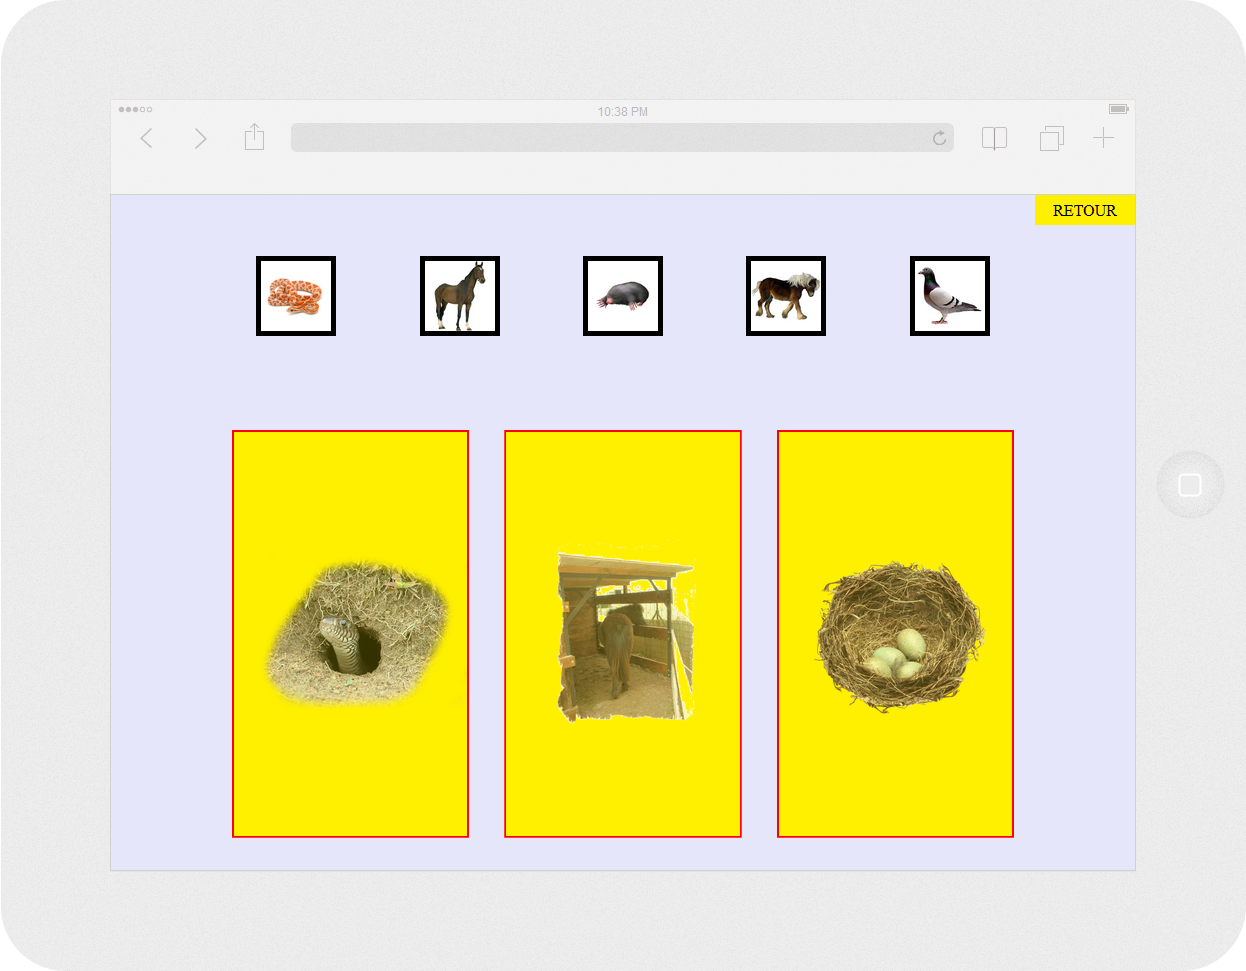
\includegraphics[width=0.6\textwidth]{page4}
\end{center}
\vspace{0.5cm}
\hspace*{0.6cm}Le dernier niveau est le plus difficile de tous. Cependant la structure et le gameplay restent l\`a aussi similaires aux deux niveaux pr\'ec\'edents. Seules les associations avec les animaux diff\`erent. Cette fois, les animaux sont tri\'es suivant leur habitats. Pour continuer avec les exemples, prenons le cheval, ce dernier vit dans une \'ecurie. On d\'eplacera donc l'image du cheval dans la case repr\'esentant l'\'ecurie.
    
\section{Sc\'enario}

Le jeu est compos\'e de deux parties. En haut (zone1 en rouge), vous trouverez les animaux que vous pouvez d\'eplacer et en bas (zone 2 en violet) les zones o\`u vous pouvez les d\'eplacer.
\vspace{0.5cm}\\
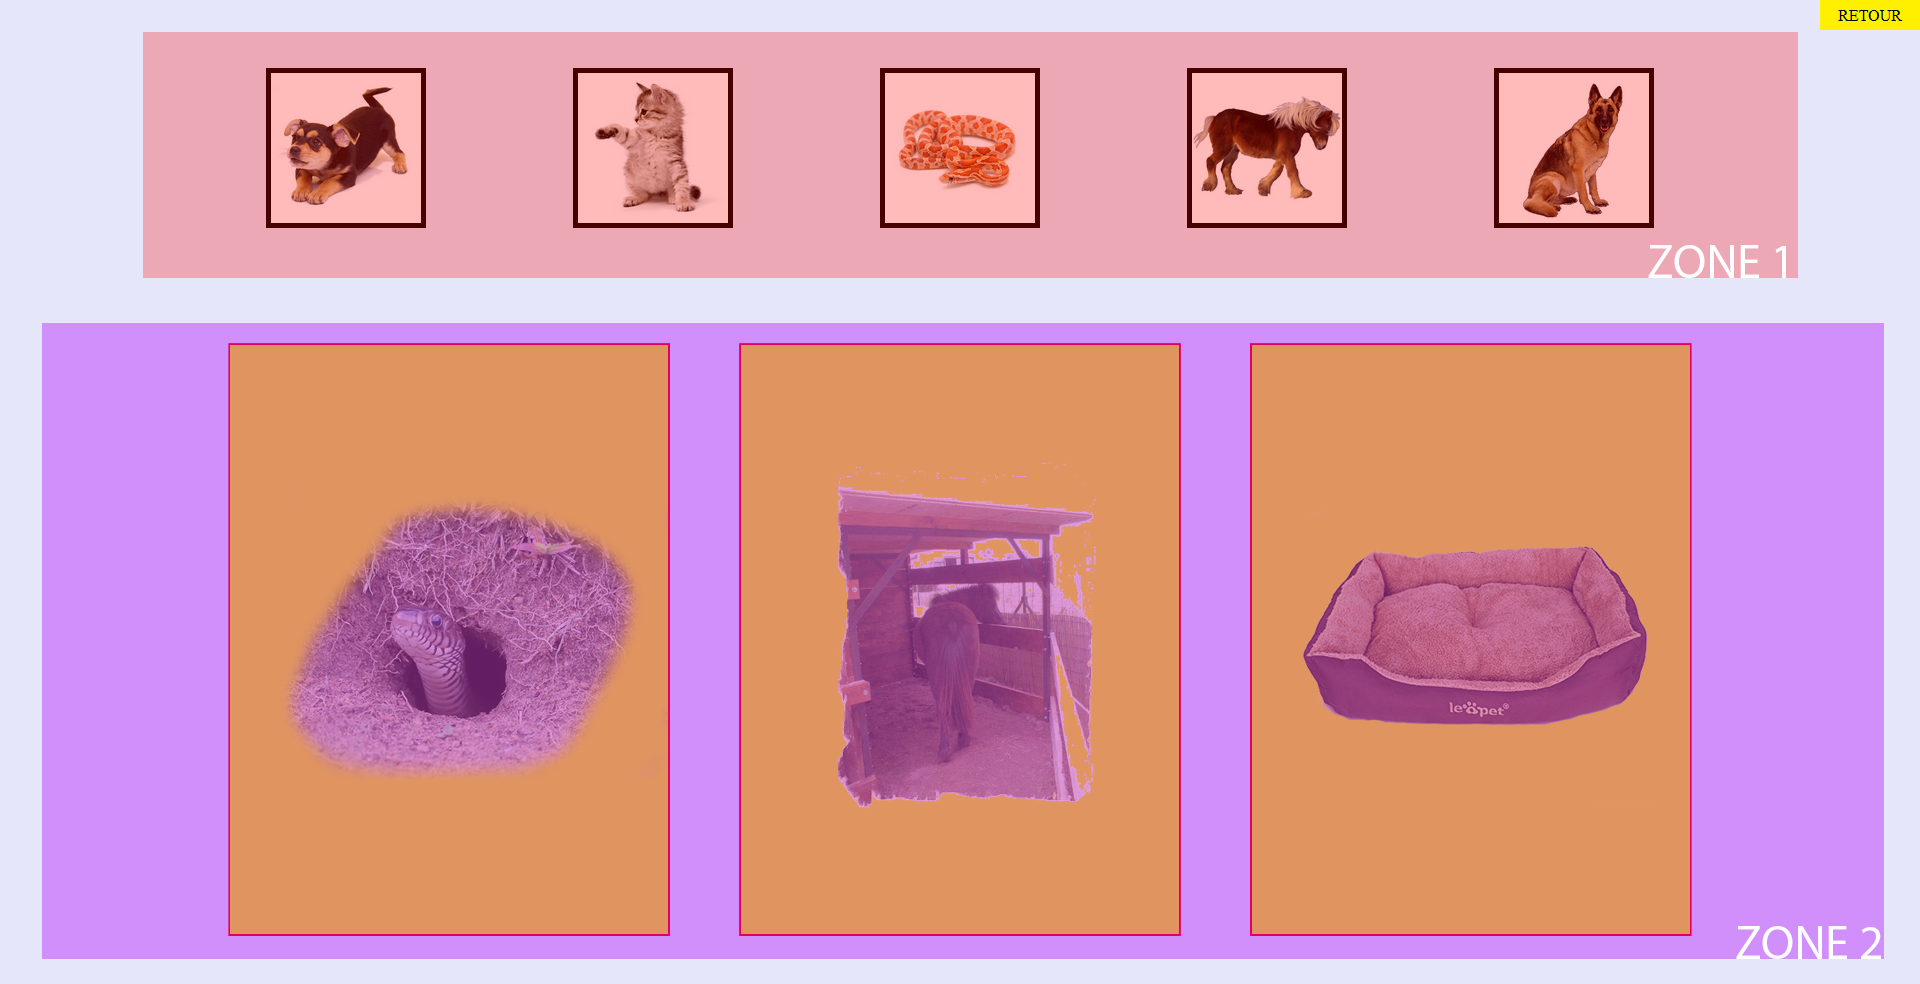
\includegraphics[width=1.0\textwidth]{zone}
\vspace{0.5cm}\\
Le but du jeu est de d\'eplacer les animaux de la zone 1 vers la zone 2 en suivant une certaine logique. Reprenons notre exemple pr\'ec\'edent et notons les animaux de la zone 1.\\
\vspace{0.5cm}\\
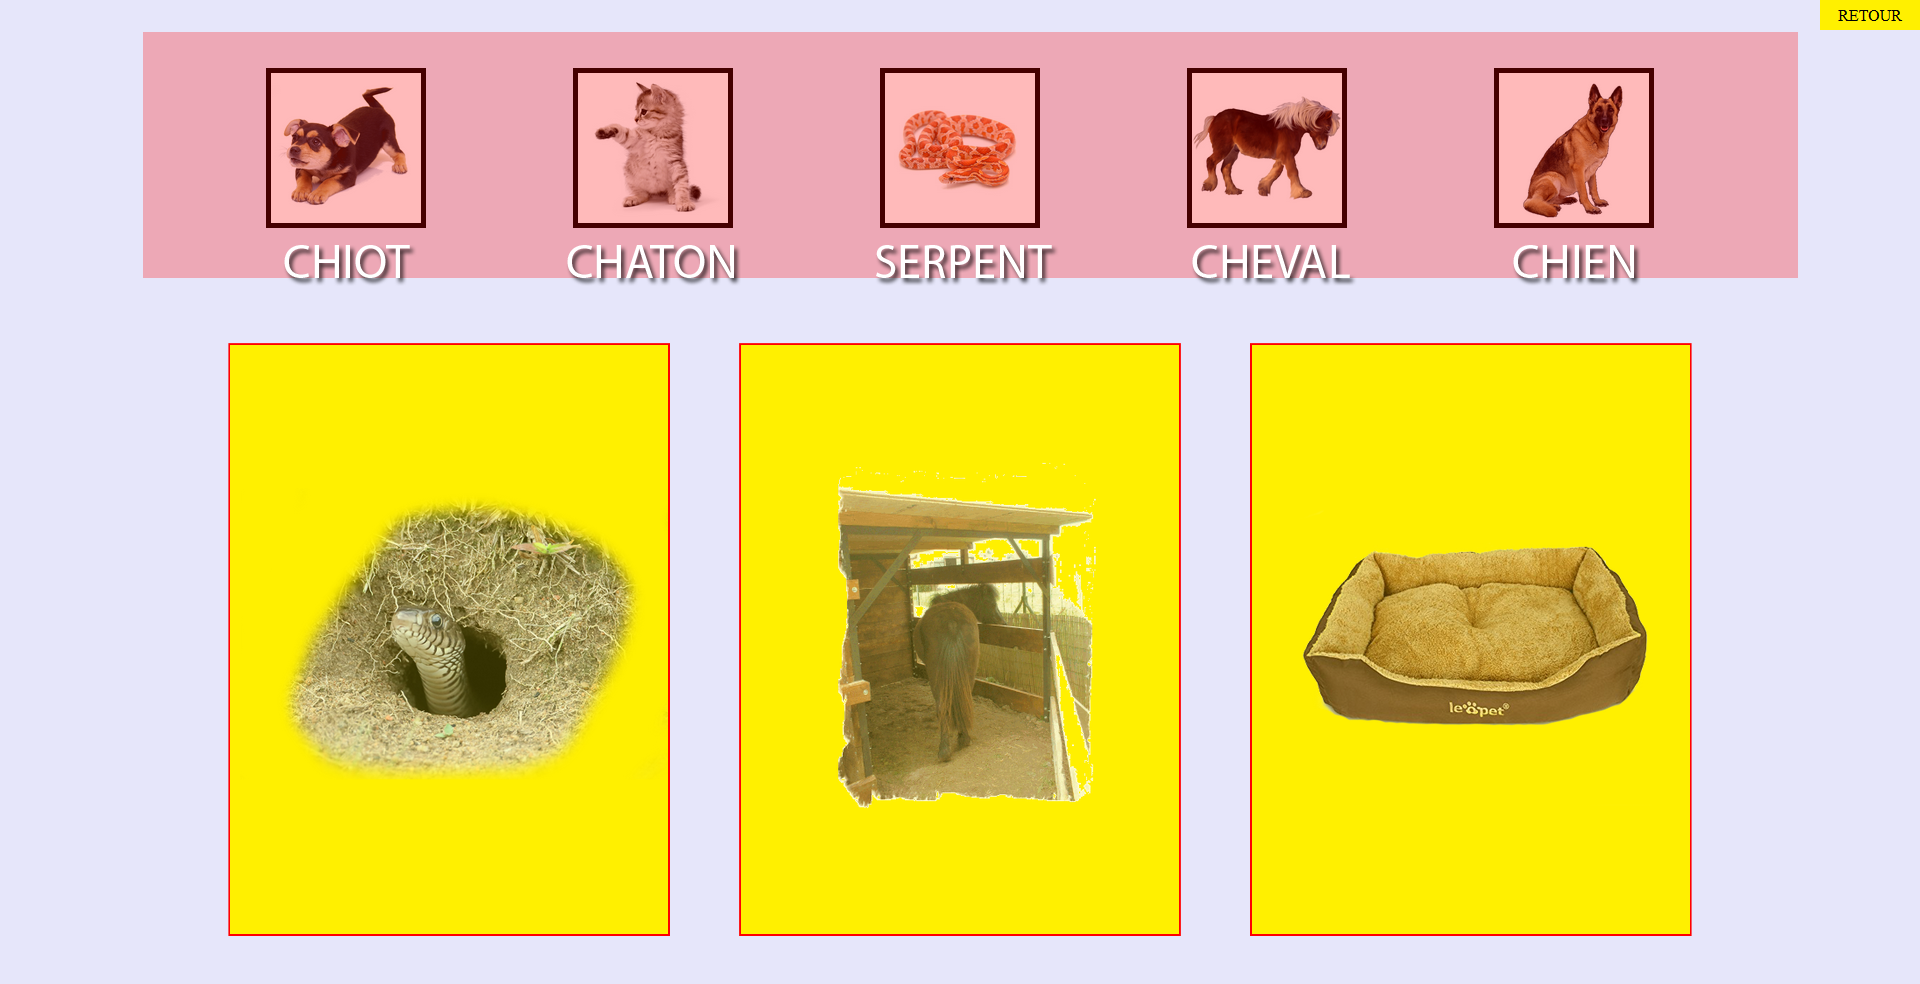
\includegraphics[width=1.0\textwidth]{zone1}
\vspace{0.5cm}\\
Prenons par exemple le cheval, nous allons cliquer dessus et maintenir notre clic tout en d\'epla\c{c}ant la souris.
\vspace{0.5cm}\\
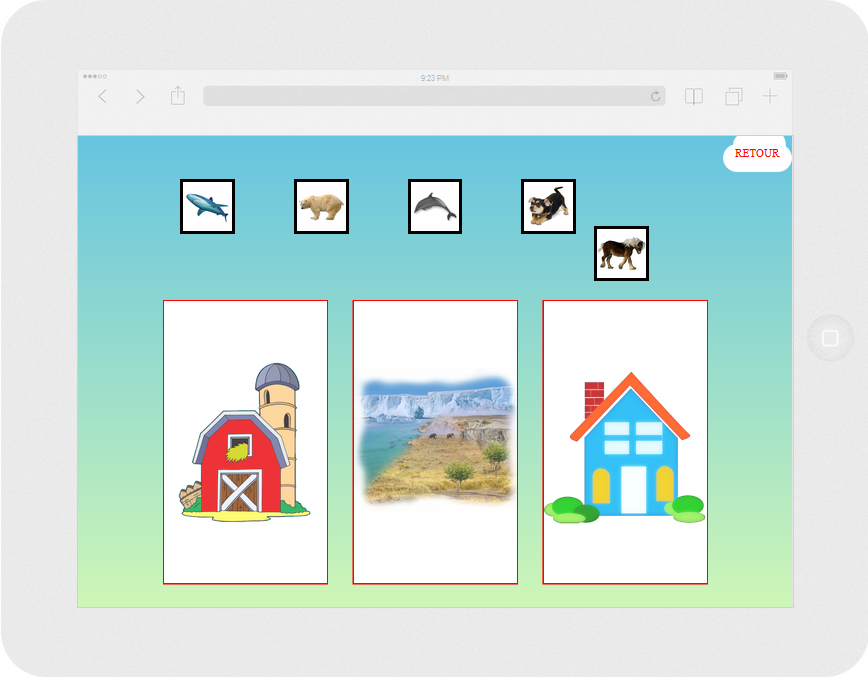
\includegraphics[width=1.0\textwidth]{zone2}
\vspace{0.5cm}\\
Si nous rel\^achons notre clic, l'image du cheval retournera \`a sa place automatiquement. Maintenant, regardons avec attention la zone 2 et d\'ecrivons l\`a aussi les images. 
\vspace{0.5cm}\\
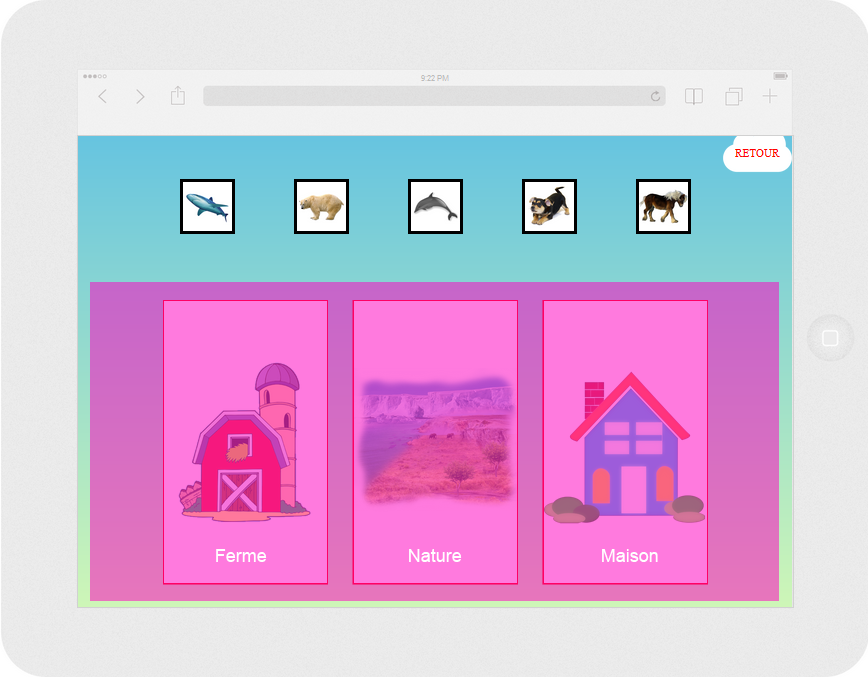
\includegraphics[width=1.0\textwidth]{zone3}
\vspace{0.5cm}\\
Reprenons maintenant notre cheval et d\'epla\c{c}ons le dans la zone qui lui correspond (l'\'ecurie). L'image se fixera alors \`a la zone et vous ne pourrez plus y toucher. Vous avez la bonne r\'eponse !
\vspace{0.5cm}\\
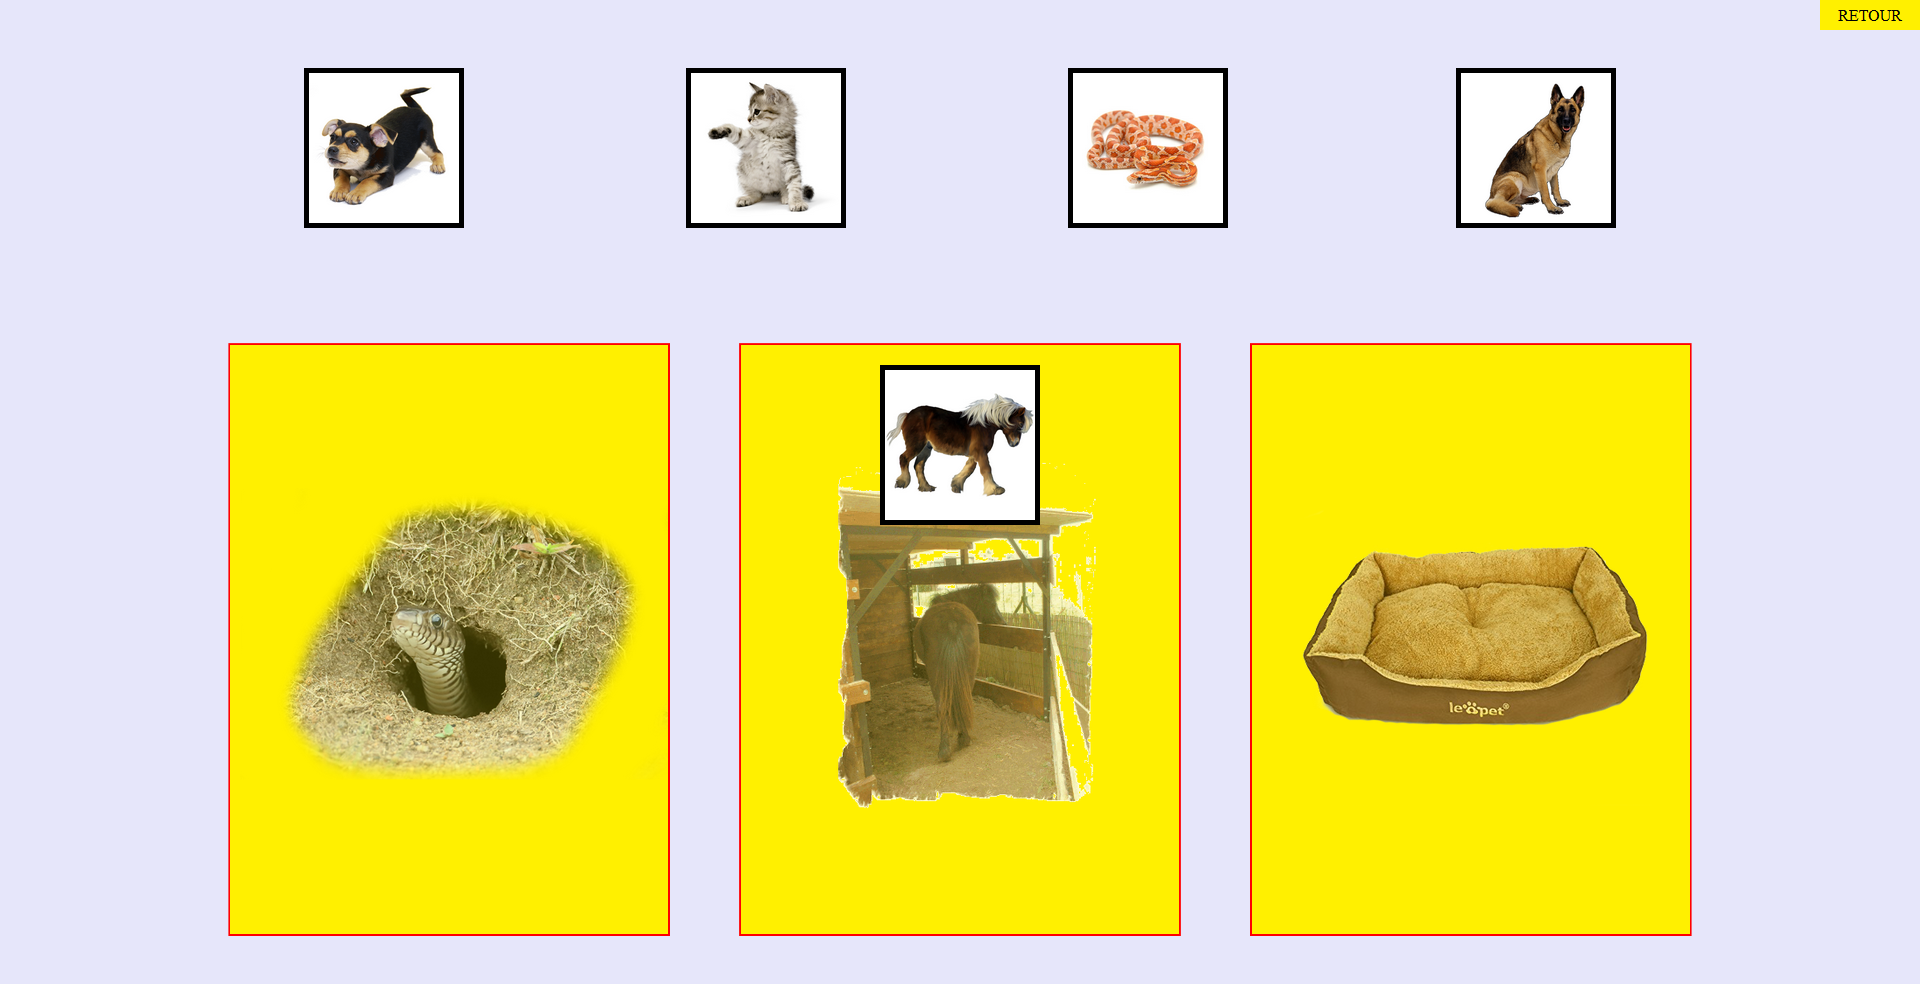
\includegraphics[width=1.0\textwidth]{zone4}
\vspace{0.5cm}\\
Maintenant effectuons cette m\^eme op\'eration pour chaque image restante dans la zone 1. Allez, encore un petit effort, nous y somme presque.
\vspace{0.5cm}\\
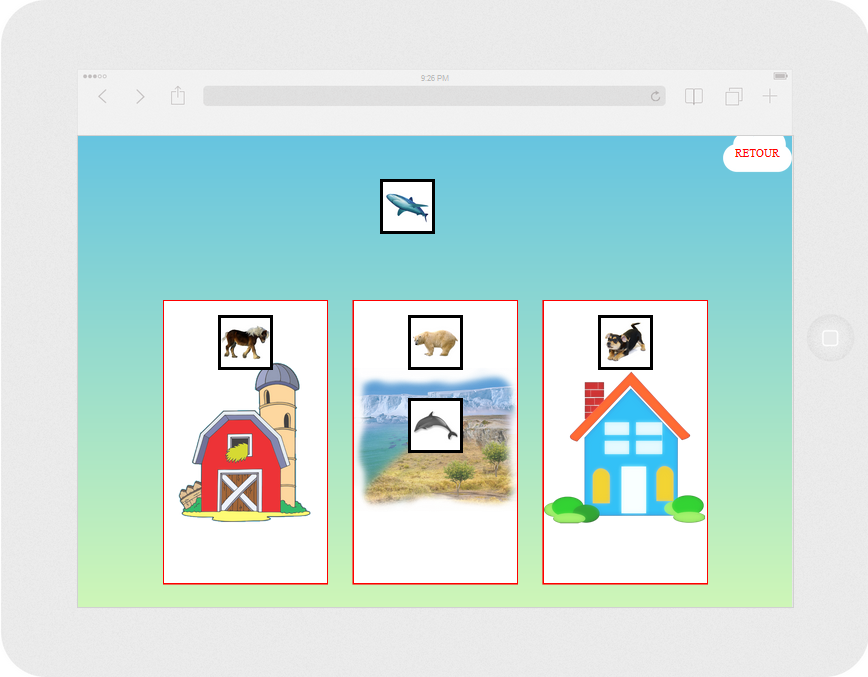
\includegraphics[width=1.0\textwidth]{zone5}
\vspace{0.5cm}\\
Si vous r\'epondez correctement en pla\c{c}ant l'integralit\'e des images, un message vous disant "Bravo" s'affiche alors pour vous f\'eliciter.
\vspace{0.5cm}\\
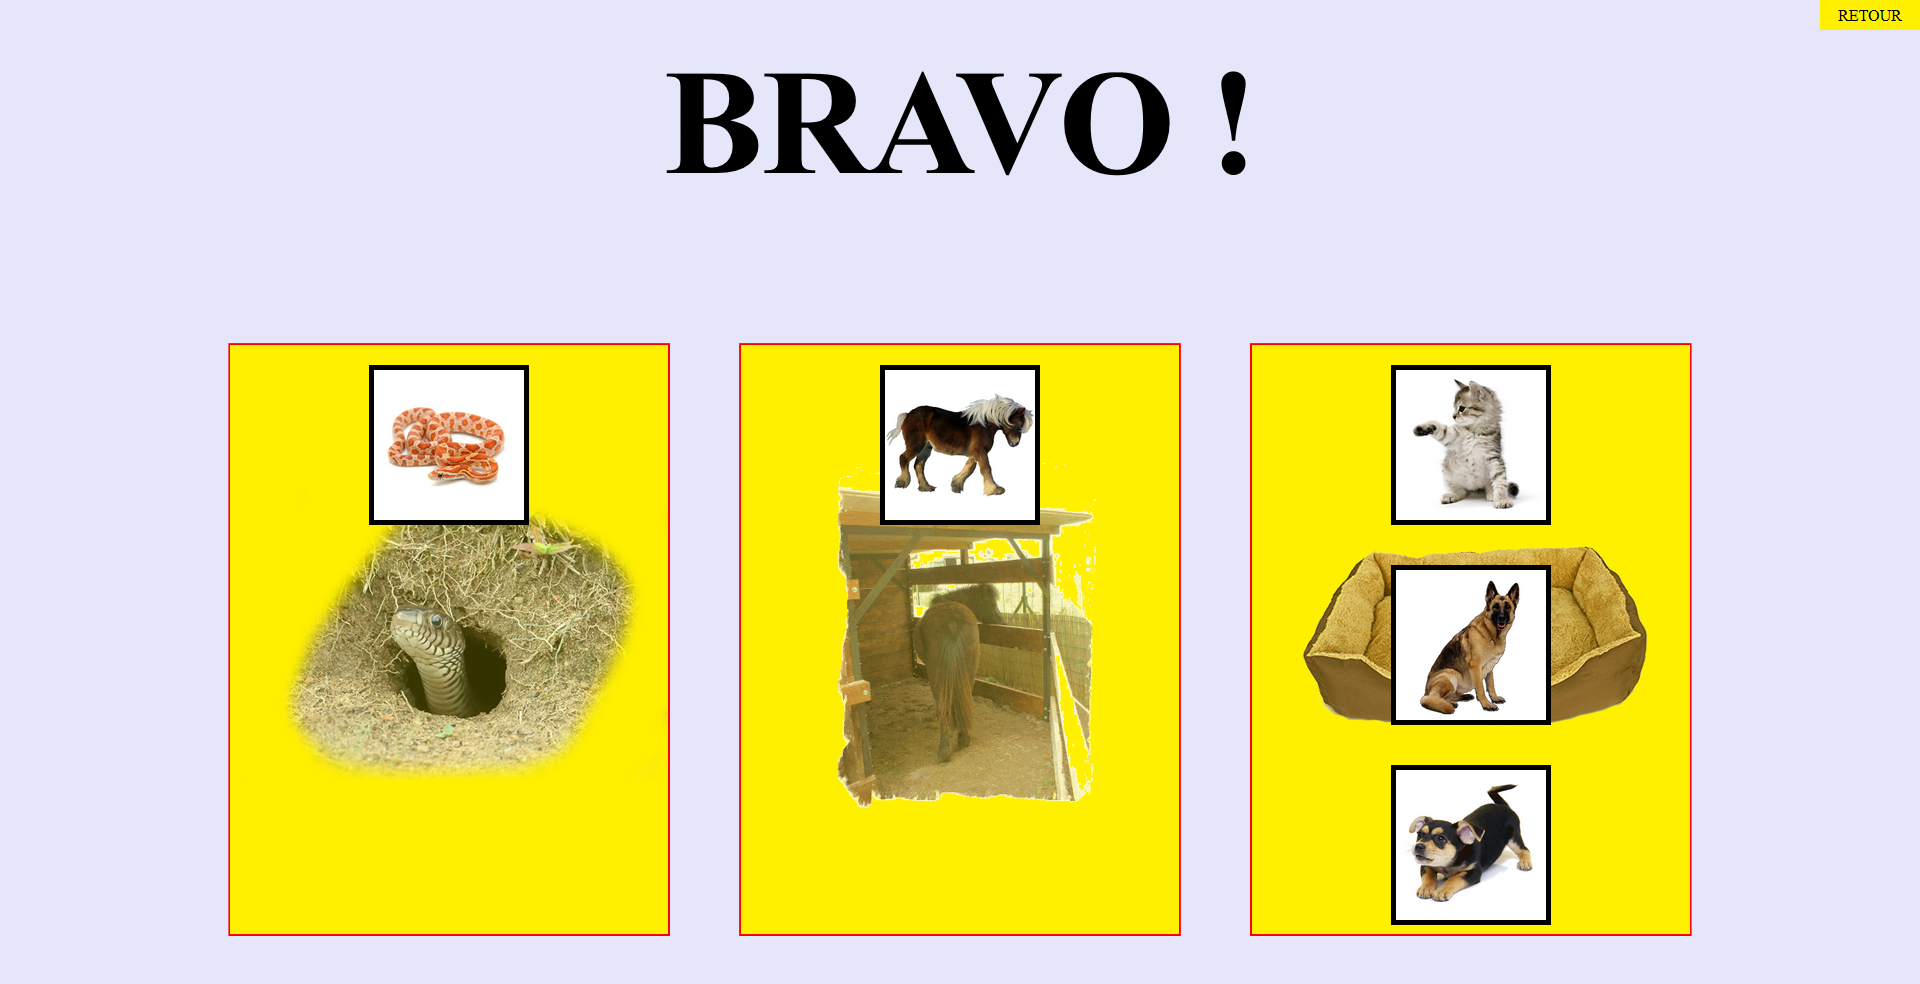
\includegraphics[width=1.0\textwidth]{zone6}
\vspace{0.5cm}\\
Puis une nouvelle partie commence avec de nouveaux \'el\'ements dans les deux zones.
\vspace{0.5cm}\\
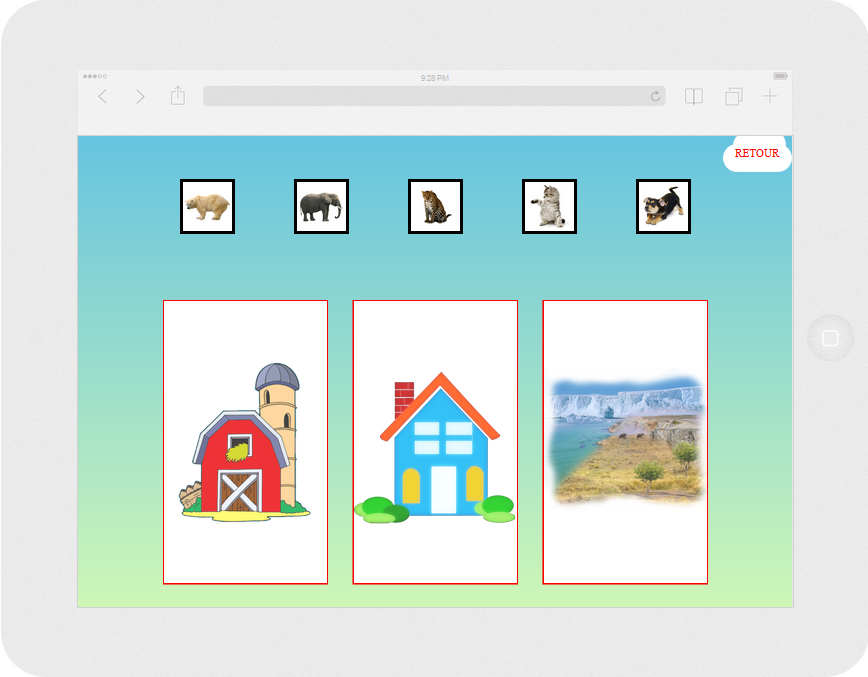
\includegraphics[width=1.0\textwidth]{zone7}
\vspace{0.5cm}\\


\section{Normes, standards et outils}

\subsection{M\'ethodes de conception}
\hspace*{0.6cm}Les m\'ethodes de conception sont utilis\'ees afin d'am\'eliorer la qualit\'e de la conception finale.
\vspace{0.5cm}\\
\hspace*{0.6cm}La norme \textbf{UTF-8} est utilis\'ee afin de rendre les textes utilis\'es universels et fiables. En utilisant cette norme, le jeu devient utilisable et surtout r\'eutilisable sur l'ensemble des ordinateurs \`a travers le monde.
\vspace{0.5cm}\\
\hspace*{0.6cm}Concernant l'\'elaboration du jeu, un style de conception ascendante a \'et\'e choisi. Cette approche permet de s'appuyer sur des scripts r\'eutilisables. Les niveaux \'etant sensiblement les m\^eme, on peux donc impl\'ementer la base du jeu dans un script que nous r\'eutiliserons dans l'ensemble des niveaux.

\subsection{Standards}

\hspace*{0.6cm}Les conventions de codage utilis\'ees sont celles approuv\'ees par le W3C. Les commentaires du Javascript qui sont dans le code suivent quant \`a eux les conventions de codage de Java.

\subsection{Langages de programmations}

\hspace*{0.6cm}L'\textbf{HTML5}, qui est la derni\`ere r\'evision majeure d'HTML, permet de repr\'esenter les pages web du jeu. Ce langage de balisage permet de structurer et de mettre en forme le contenu du jeu.\\
\hspace*{0.6cm}Le \textbf{CSS4} permet de d\'ecrire la pr\'esentation de notre jeu comme par exemple la taille de la police, la taille des images...\\
\hspace*{0.6cm}Le \textbf{JavaScript}, qui est le langage de programmation de script par excellence, permet d'ajouter de l'interaction au jeu. Ce langage permet entre autre d'interagir avec le clique lorsque l'on d\'eplace les images des animaux.\\
\hspace*{0.6cm}Le \textbf{XML} permet dans le jeu d'ajouter ou de supprimer des animaux facilement sans modifier une seule ligne de code.

\subsection{Environnement et outils de d\'eveloppement}

\hspace*{0.6cm}Les diff\'erentes versions du jeu seront visionnables, t\'el\'echargeables sur un \textbf{GIT}, un logiciel de traitement de versions d\'ecentralis\'e. Cet outil permet aux membres de l'\'equipe de d\'evelopper chacun une part du code final et de l'\'echanger facilement. Le code sera aussi visible par toute personne ext\'erieur au projet. Un retour d'une personne ext\'erieure serait un plus qui pourrait am\'eliorer le jeu et/ou le code.
\vspace{0.5cm}\\
\hspace*{0.6cm}\textbf{JQuery}, une biblioth\`eque de Javascript, permet de faciliter la conception des scripts du jeu. Cette biblioth\`eque gr\^ace \`a des fonctions d'animations ou d'\'ev\'enement d\'ej\`a impl\'ement\'e permet donc de gagner du temps. Le d\'eveloppement est par cons\'equent acc\'el\'er\'e.
\vspace{0.5cm}\\
\hspace*{0.6cm}Enfin, les images du jeu sont en grande partie issus d'internet avec quelques modifications l\'eg\`eres r\'ealis\'e avec \textbf{Photoshop}. 

\subsection{Outils de test}
\hspace*{0.6cm}Pour tester le jeu, les diff\'erents navigateurs sur le march\'e (\textbf{Google Chrome, Mozilla Firefox, Safari, Opera, Internet Explorer}) seront amplement suffisants car ces derniers disposent d'outils permettant d'effectuer des tests et de d\'eboguer les applications.\\
\hspace*{0.6cm}Pour les tablettes, \textbf{Opera Mobile Emulateur} est un outil puissant permettant de reproduire le comportement des tablettes et t\'el\'ephones.\\

\section{Planning}

\begin{tabular*}{1.0\textwidth}{@{\extracolsep{\fill}} | c | l | }
  \hline
  & Choix du sujet\\
  & Cr\'eation du dossier de conception\\
  Semaine 1 & Cr\'eation du premier prototype\\
  & \'Ecriture de la documentation\\
  & Test de la version 1.0\hspace*{7.6cm}\\
  \hline
  & Ajout de nouvelles id\'ees\\ 
  Semaine 2  & Am\'elioration du prototype jusqu'\`a la version finale\\
  & Test des versions intermediaires\\
  \hline
  Semaine 3  & Test et finalisation graphique\\
  \hline
  & Correctifs des d\'etails\\
  Semaine 4-7 & Ajout de donn\'ees\\
  & Tests finaux\\
  \hline
\end{tabular*}

\begin{center}
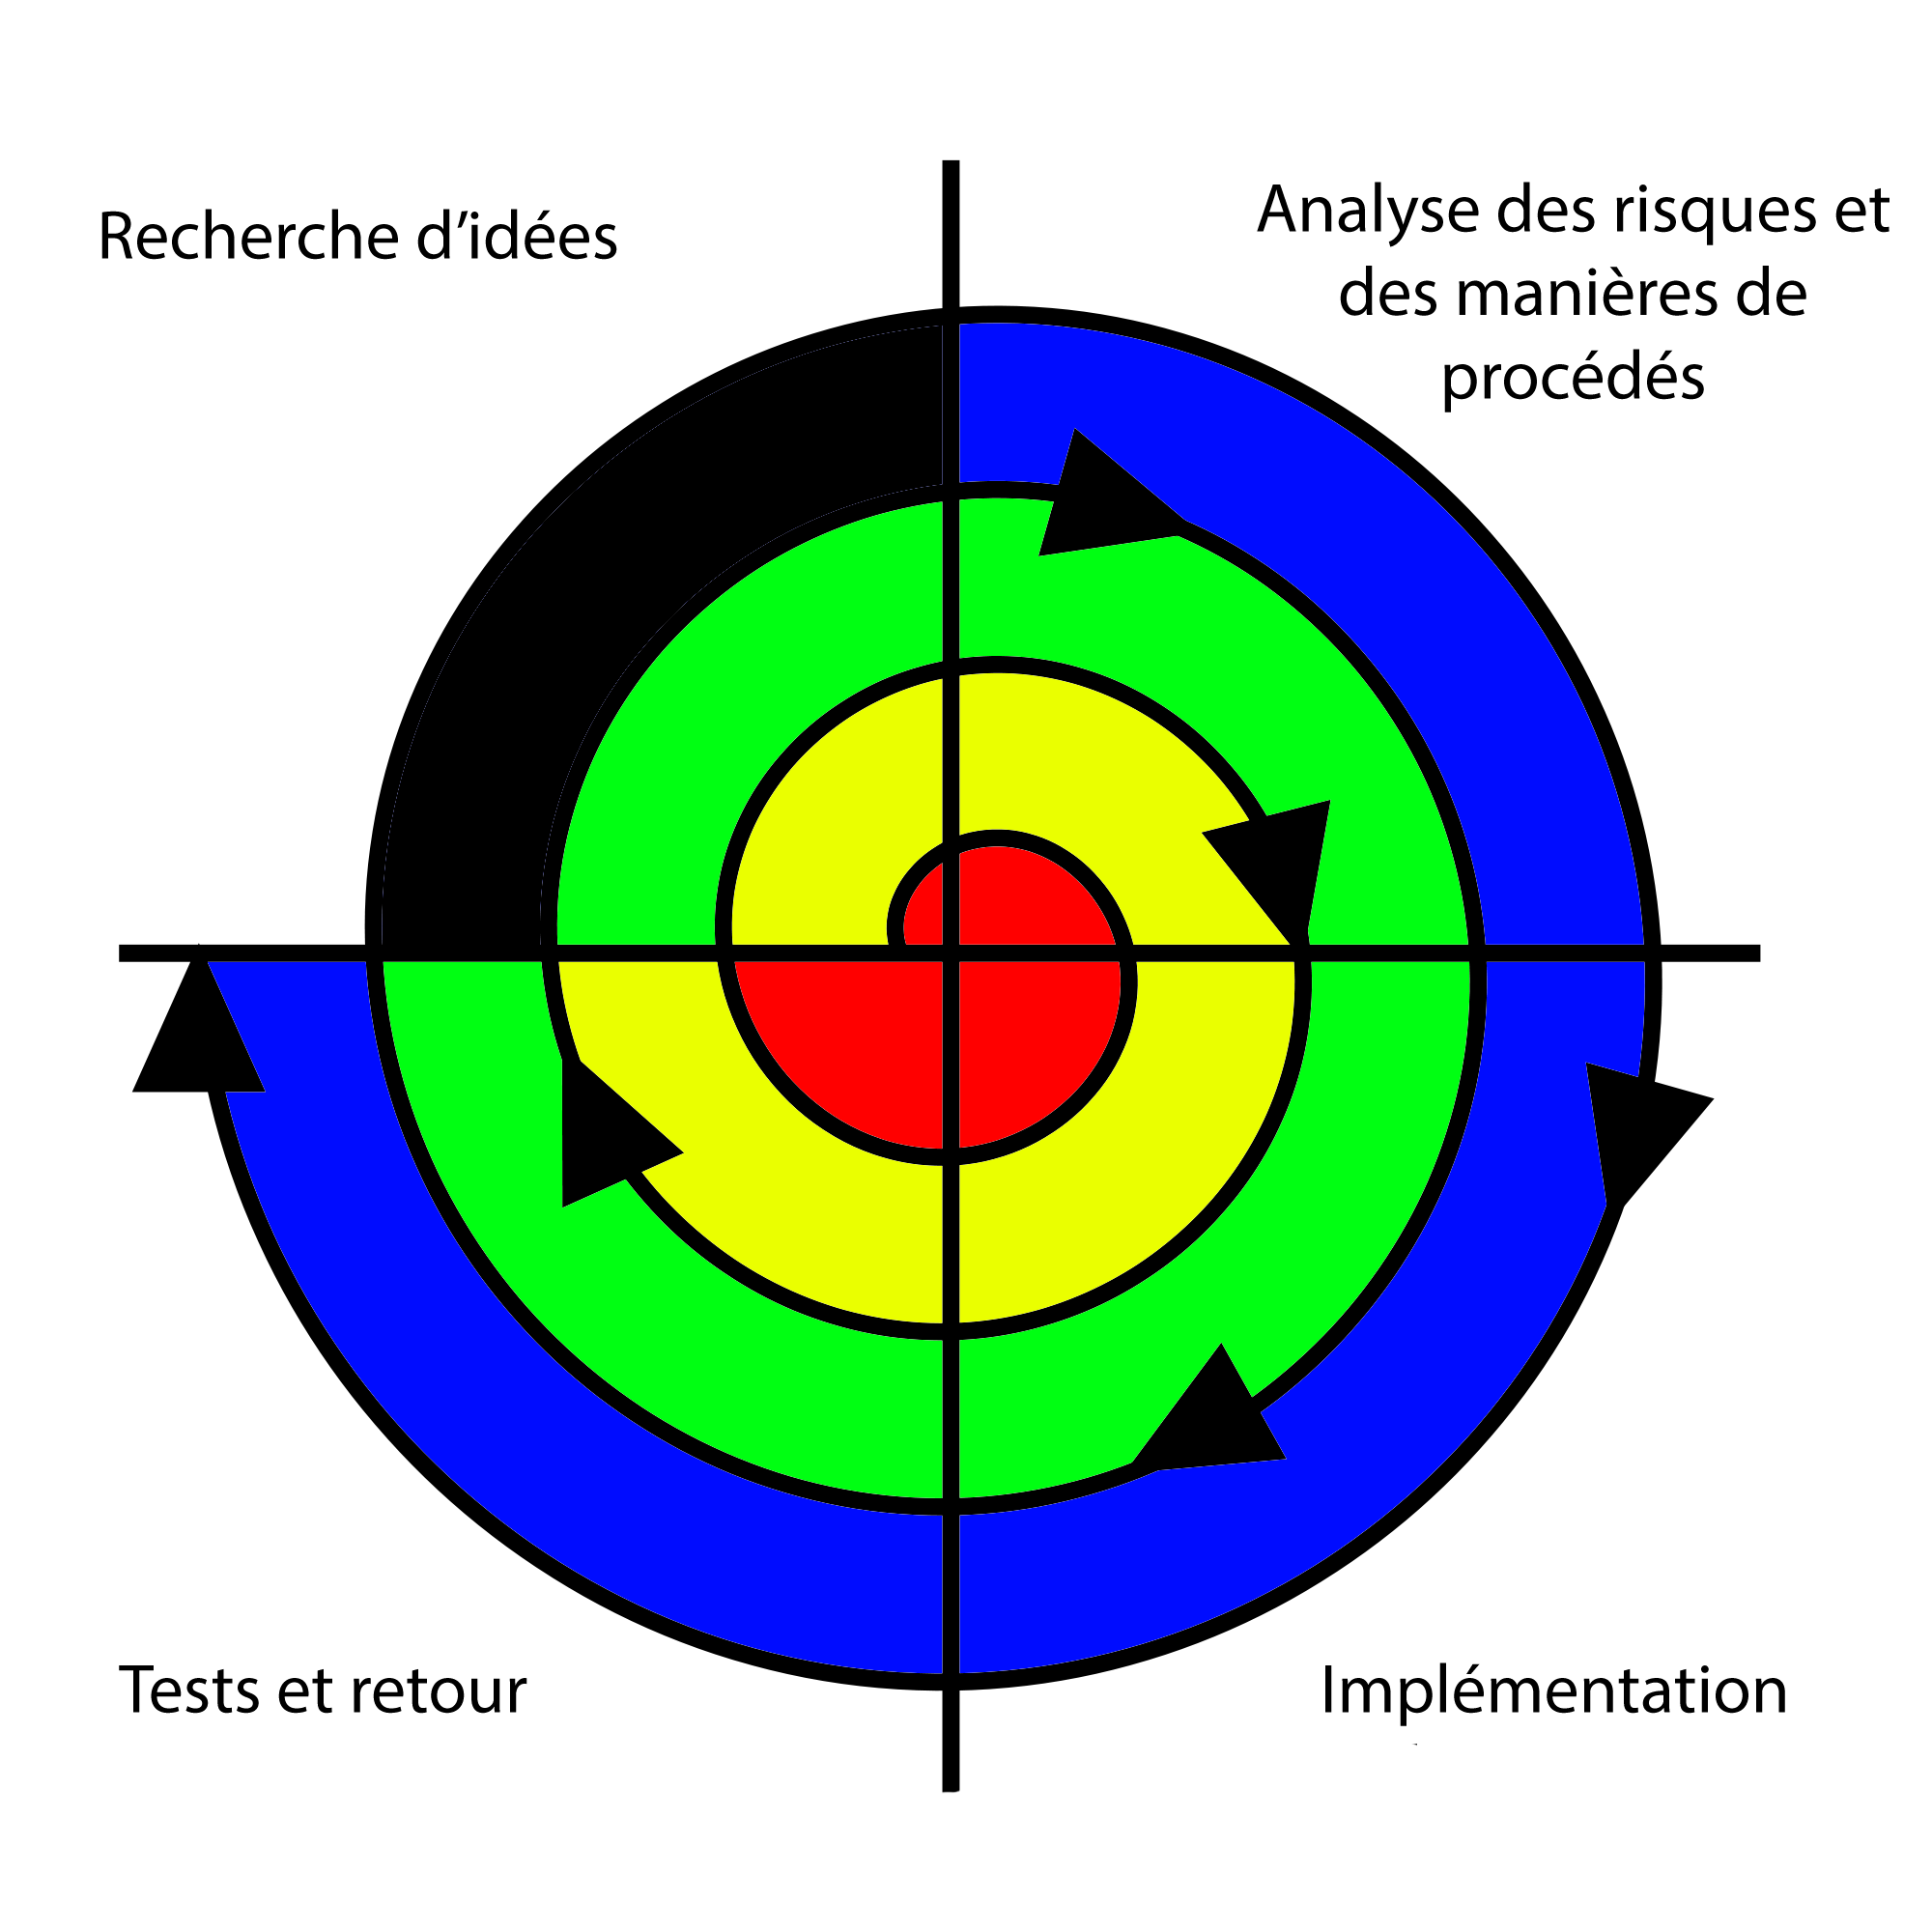
\includegraphics[width=0.6\textwidth]{spiral}\\
\end{center}

\textit{Le mod\`ele spirale est un mod\`ele de cycle de d\'eveloppement par impl\'ementation de version successives, le cycle recommence en proposant un produit de plus en plus complet. On distingue quatres phases dans le d\'eroulement du cycle en spiral :
\begin{itemize}
  \item Recherche d'id\'ees
  \item Analyse des risques et des mani\`eres de proc\'ed\'es
  \item Impl\'ementation
  \item Tests et retour
\end{itemize}
}
\vspace{0.7cm}
\hspace*{0.6cm}On suivra ainsi un mod\`ele spirale pour le d\'eveloppement. En rouge, on retrouve notre premi\`ere semaine de d\'eveloppement. \`A l'instant o\`u ces lignes sont \'ecrites, un premier prototype a \'et\'e test\'e et produit. La semaine 2 en jaune sera donc de l'ajout d'id\'ee avec l'impl\'ementation et les tests qui iront avec. La semaine 3 en verte suivra le m\^eme sch\'ema et pourra, suivant le d\'eroulement du projet, se reproduire une ou deux fois. Puis la derni\`ere semaine en bleu sera celle o\`u plus aucun ajout ne sera tol\'er\'e.\\


\end{document}